\chapter{SCOBY Machine \& Materials}


\section{Overview}

In the same way as for the environent control project with the scoby, we had to think about how machines can help us make this new material our own, in much the same way as 3D printers popularized the use of PLA. 

The methods and machines presented here are designed to facilitate the use of this biomaterial, with the aim of optimizing the production of bacterial cellulose and changing the growing conditions to produce 3D cellulose. 

In addition, unlike mycelium, which unfolds in a substrate contained in a mold, cellulose requires more attention to shape channelling, both for molding and demolding. 

% \begin{figure}[h]
%     \centering
%     \includegraphics{images/Myceliummachine.png}
%     \caption{System design representation}
%     \label{fig:}
% \end{figure} 

\section{Systems design}
The bioreactor takes the form of a closed space like a box, with openings covered with microporous plaster to allow air to pass through without contaminating the space. Into which the culture medium can be introduced.

% \begin{figure}[h]
%     \centering
%     \includegraphics{images/Myceliummachine.png}
%     \caption{System design representation}
%     \label{fig:}
% \end{figure} 



\section{Manufacturing Processes \& Grow Theory}


the manufacture of bacterial cellulose cookers comprises two stages: preparation of the culture medium and manufacture of the bioreactor to house the culture medium. 
the preparation of the home-made culture medium proceeds as follows:
freshly crushed bacterial cellulose is introduced into a mixture of tea, water, sugar and vinegar. 


\begin{figure}[h]
    \centering
    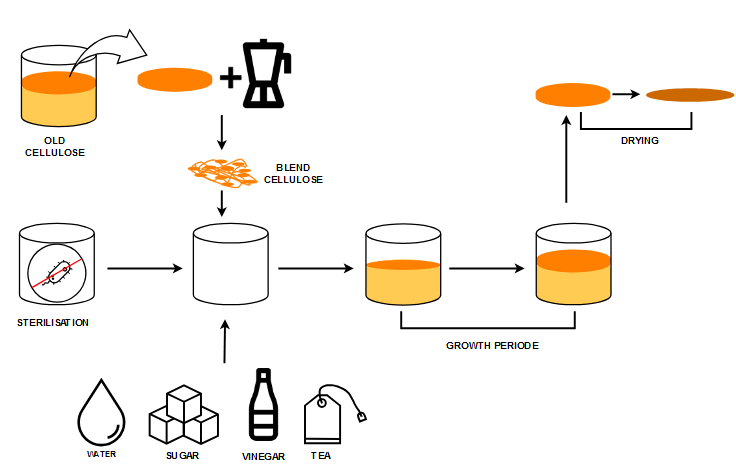
\includegraphics{images/SCOBY_diag.png}
    \caption{Classical manufacturing processes}
    \label{fig:}
\end{figure} 

\section{Contribution}

\subsection{Rotary Bioreactor}


\section{Result}

